\chapter{Evaluation}

In order to evaluate the performance and correctness of our proposed GMM and PCA-based anomaly detection methods, we have trained and tested the models against the set of data provided by \textbf{"PolyEnergyNet – Resiliente Polynetze zur sicheren Energieversorgung"}. We started the analysis by grouping the datasets into weekday and weekends in order to identify the patterns of these two groups separately. We believe the patterns to differ significantly between the weekday and weekends. \\

\section{PCA}

We start the evaluation of PCA based anomaly detection method by briefly specifying the steps involved in preprocessing and then dive into describing the performance of our PCA based anomaly detection method. The preprocessing for PCA based anomaly detection will be done as follows:
\begin{itemize}
\item\textbf{Data Smoothing:} In order to clearly reveal the underlying trends and seasonal variations of our time series data we apply the simple "moving average" as our data smoothing method. This moving average will smooth the random variation or we can say, the noise in the data by taking average of values over the given window period. Moving average works better when using data which are measured equi-distantly, by equi-distantly we mean, all the observations are taken at equal time intervals i.e every second data. We use window size = 60 which corresponds to one minute of our data. All the variations such as for example, a sudden dip in the phase displacement(CosPhi value) which might have occured due to incorrect sensor readings will be smoothed.

\item\textbf{Normalization:} The smoothed data is normalized by removing the mean of each column and the difference to mean is stored as the normalized value. What we are doing here is scaling the values of each column of our dataset to represent mean 0 and unit variance. Our data contains columns such as voltages, current, power, phase displacement values and these values are not measured against a single unit, that is, voltage values are in Volts, current values are in Amperes, power values are in Watt-hour and phase displacement are in Degrees. If we do not normalize this data then the result of PCA for choosing the right number of components will not be accurate. By right number of components we mean that the components may represent variances captured by columns which contain larger values. In our dataset we see that, power values are in the range of thousands to hundreds of thousands, voltages are in range of 200 to 270, current are within 100 to 150, where as phase displacement values are within 1. 

Without normalizing we tend to obtain components of largest values like variances of  power and/or voltages  as high variance since their values are very large and the phase displacement values which are too low can be neglected. To account for this, we scaled the values such that each column had mean of 0 and variance of 1, this ensured that the variance in all the columns are retained and made sure PCA will consider all the necessary features and thus the components we choose after applying PCA were correct when it comes to identifying the right number of components.
\end{itemize}

\begin{figure}
\centerline{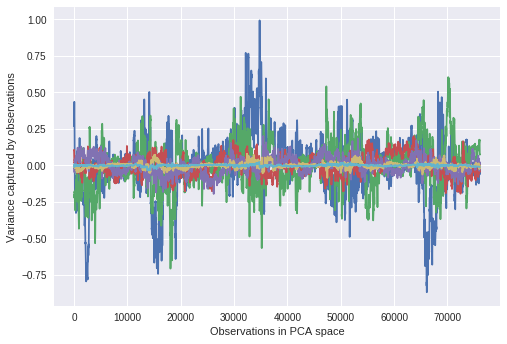
\includegraphics[totalheight=8cm]{PCA_fit.png}}
    \caption{This diagram shows the distribution of data across PCA space. The feature in blue captures the most variance in all the observations as you can see in the figure. The feature represented in green captures the next highest variance whereas the variances which are measured too low by PCA can be seen by the observations in light blue, magenta and red which are almost 0 and forms the residual subspace. X-axis represents the number of observations and y-axis captures the variances of each feature according to the measured observations.}
    \label{fig:pca}
\end{figure}

\textbf{Extracting relevant features:} Once the data is smoothed and normalized, the next step we carried out was to divide all the features based on the amount of variances captured by applying PCA . Our aim here was to group the features into two subgroups which we call as normal subspace and residual subspace. Normal subspace is composed of components capturing the major variances and residual subspace is composed of components capturing the minor variance which are usually ignored. Our contribution will be researching in this residual subspace as we assume any anomalous data will be captured by this residual subspace and then we define a threshold value above which, we term the data points as tagged as anomalous points. 
   
\begin{figure}
\centerline{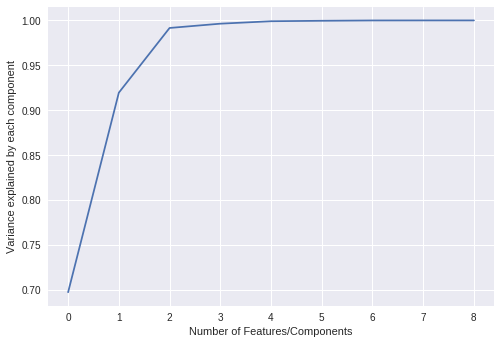
\includegraphics[totalheight=8cm]{PCA_cusum_variance.png}}
    \caption{This graph shows the cumulative sum of PCA explained variance. The x-axis corresponds to number of features considered for constructing the PCA and the y-axis denotes the cumulative sum of variances captured by components. The y-axis has values from 0 to 1 with 1 indicating 100\% variance.}
    \label{fig:PCA_cusum_variance}
\end{figure}

\textbf{Threshold:} An optimal threshold is defined to distinguish between normal and anomalous data. As discussed earlier while describing our PCA based anomaly detection method, we define a threshold value derived from calculating Squared Prediction Error. All the values above this threshold are considered as anomalies. 

\textbf{Results:} We fit the PCA model for all the 9 columns of our data and transform our data to PCA axes. 
\begin{figure}
\centerline{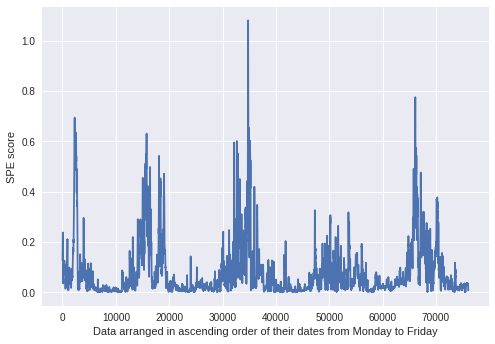
\includegraphics[totalheight=8cm]{SPE_error.png}}
    \caption{Results of SPE Error value against the data. This figure shows the distribution of each day's data. Week's all five working days SPE calculated value is shown as five different distribution in the plot. Each distribution separately corresponds to each day's electricity usage pattern of the area under consideration. Spikes in the third and fifth distribution are the largest spikes with bigger Square Prediction Error(SPE) value.}
    \label{fig:spe}
\end{figure}The resultant PCA model divided the data into two orthogonal subspaces namely, normal subspace and residual subspace. Normal subspace is constituted of 'n' components based on the percentage of variance we wish to retain. The percentage of variances are nothing but the eigen values of the corresponding n components. The results of fitting our data with PCA is better explained by the measure "cumulative sum of explained variance ratio" as shown in the Fig \ref{fig:PCA_cusum_variance}. From the figure, we can explain the variances of all components. Component 0 which is the first component captures 70\% of the variance or has the largest eigen value, component 1 together with component 0 captures about 91.9\% variance, component 2 added  to the first two will account for 99.1\% and so on. 

We had to play around with our experiments to come up with the right amount of residual space taking into consideration how much variances should we capture in normal subspace and how much variance should be allowed to retain in residual subspace. We evaluated starting from two components explaining 91.9\% through five components explaining 99.9\% of variance.\\


\section{GMM}

We follow a similar procedure as we followed for PCA based approach. The GMM based anomaly detection results when compared to PCA based methods were quite satisful and we were able to detect both the injected anomalies and the unusual behavioral data in our dataset.

\begin{itemize}
\item\textbf{Dataset and preprocessing:} We took same one weeks data from Monday to Friday which we used for PCA as well. This data was subjected to filtering and data smoothing similar to the steps followed under PCA. In order to account for equal variability the dataset had to undergo dimensionality reduction for which we used the principal component analysis. From the variance explained by each component we made a decision to use first three prinicpal components which were able to capture 99.9\% variance as can be seen in the Fig \ref{fig:PCA_cusum_variance}.

\begin{figure}
\centerline{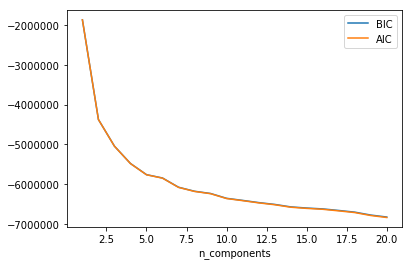
\includegraphics[totalheight=8cm]{BIC_AIC.png}}
    \caption{BIC score for the data. Applied on the data to determine the number of clusters to be used. The point at which the BIC value is lower is considered as the number to be used as the number of clusters. The plot has a lower value at cluster number = 20. }
    \label{fig:bic}
\end{figure}

\item\textbf{Model the data:} The data was fitted using the Gaussian Mixture Model function readily available with the python package of scikit learn. To efficiently model our data and to understand the underlying behavior using GMM, we had to carefully choose the fitting parameters. Model selection is done using the Bayesian Information Criterion as shown in the Fig \ref{fig:bic}.  We measure the correctness and the perfectness of our model by carefully looking at,  the \textit{number of clusters}. 

Cluster number will determine how well our GMM will fit our data. GMM uses the Expectation-Maximization algorithm as described earlier in our work to assign data points to the clusters. If the clusters are too less, then the model will underfit the data constraining all the data points into these small clusters and if the number of cluster is too high, then data which are closely related could be placed in different clusters leading to overfitting of the data. To handle this condition of overfitting and underfitting we use Bayesian Information Criterion(BIC) score to estimate the right number of clusters. We chose 50 as the initial cluster number and gradually reduced in steps of 10 keeping in my mind of the overfitting criteria and finally came down to use 20 as the number of clusters to GMM.

The advantage of using Bayesian Information Criterion is, it does not require the prior information of the data and does not even need to train the model to come up with right number of clusters. It uses a penalized maximum likelihood model selection criterion which reduces the complexity, where BIC favors the model which maximizes the BIC values.

\begin{figure}
\centerline{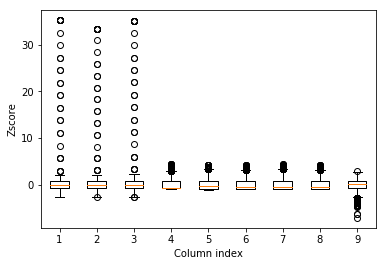
\includegraphics[totalheight=8cm]{Boxplot_Zscore.png}}
    \caption{Box plot depicting the injected anomalous data}
    \label{fig:bic_zs}
\end{figure}
\item\textbf{Results:} The results obtained using GMM on our electrical data is visualized in Fig \ref{fig:bic_zs} and Fig \ref{fig:ss}. Fig \ref{fig:bic_zs} visually illustrate many points outside the boxplot's inter-quartile range with unfilled circles. These points are clearly anomalous in nature compared to other data points which fall within inter-quartile range. The unfilled circles formed by the unusual data points are results of injecting anomalies into our data using the anomaly tool developed and described earlier. For our model to perform better it should be able to identify these injected points and classify them as anomalous. 

The score samples are the measure of weighted log probabilities of the data points obtained after fitting the test data injected with anomalies to GMM. The points are plotted in the form of histogram as expressed by Fig\ref{fig:ss}. We calculate the confidence intervals from the obtained score sample values of each data point. With the assumption of data following Gaussian distribution, we go by defining an optimal threshold value based on percentage of confidence intervals we wish to retain and standard deviation measure.

We considered weighted log probabilities or score samples as a measure to distinguish between normal data and abnormal data. Normal data are the points which have high score sample values, that is values closer to 0 and all the points which tend to move away from 0 have very low probability score. Thereby limiting these low probability values to be equal to some threshold, we derive a margin and say all the points falling above this margin as anomalous. 

Carefully defining the threshold was the main aim after we have our model ready for detection. We incorporate some of the important statistical measures for our needs to explain the threshold value, such as confidence intervals, standard deviations. In common statistical process, we consider 3 standard deviation's value, collectively representing 99.73\% of points belonging to normal distribution. Here as well in our work, we use standard deviation value and tweak its value to obtain the best threshold which can easily distinguish between points of low and high probabilities.

With 2.5 times standard deviation and confidence interval of 95\% we obtained a threshold value equal to 11.099 which was sufficient enough to determine and detect the value as anomaly. Our test data had 76000 observations and without any injections we found to have 81 points which our model detected as anomalous points. These points which were detected may be caused due to faulty measurements occurred while reading the electrical units. We assume it to be faulty because the measured values when we inspected manually were found to be very unusual such as very low phase displacement values(CosPhi is the column name in our dataset), without change in any other columns(like voltages or current or power).

From now on, everytime we calculate the count of number of anomalies detected by our model to be the count as result calculated currently minus 81 which we saw in the original dataset. We inserted anomalies manually as well as with our injection tool. With the manual injection we were able to detect all the manually injected anomalies, this was obvious since we had changed the voltages and current units to a value which looks really obvious to anyone looking at the data itself. So we are happy with the first step of detection process in obvious looking anomalies. The next step was to insert anomalies with our injection tool. We started with initial injection of only few points in the range of 10 and with an increase of  40\% to the midpoint chosen as the point of injection. We remind you, the anomalies are inserted on either side of this mean point, count will determine the number of points on either side of mean is affected and the share of these points are with respect to the mid point.

The results show that our method was able to efficiently detect these points as well. The detection was not 100\% since the values are increased with a pattern as discussed previously, that is the value increases slowly upto the mean and gradually decreases after the mean. Since there is only small variation to the data points which are at the extreme ends of the point chosen for insertion, we believed our model to not detect these points. And fortunately, we were able to detect the points which were closer to the extreme ends, infact 6 to 8 observations out of 10 were detected with confidence intervals of 95\% and standard deviation of 2.5. 
\begin{figure}
\centerline{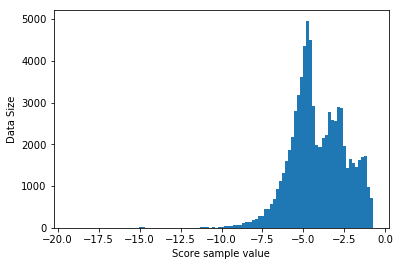
\includegraphics[totalheight=8cm]{Score_samples.png}}
    \caption{Weighted log probabilities for the data}
    \label{fig:ss}
\end{figure}

\end{itemize}

\label{sec:Eval}
